% Set the overall layout of the tree
\tikzstyle{level 1}=[level distance=1.0cm, sibling distance=4.5cm]
\tikzstyle{level 2}=[level distance=1.5cm, sibling distance=2.5cm]
\tikzstyle{level 3}=[level distance=3.0cm, sibling distance=2.0cm]

% Define styles for bags and leafs
\tikzstyle{bag} = [text width=4em, text centered]
\tikzstyle{end} = [circle, minimum width=3pt, fill, inner sep=0pt]

% The sloped option gives rotated edge labels. Personally
% I find sloped labels a bit difficult to read. Remove the sloped options
% to get horizontal labels. 
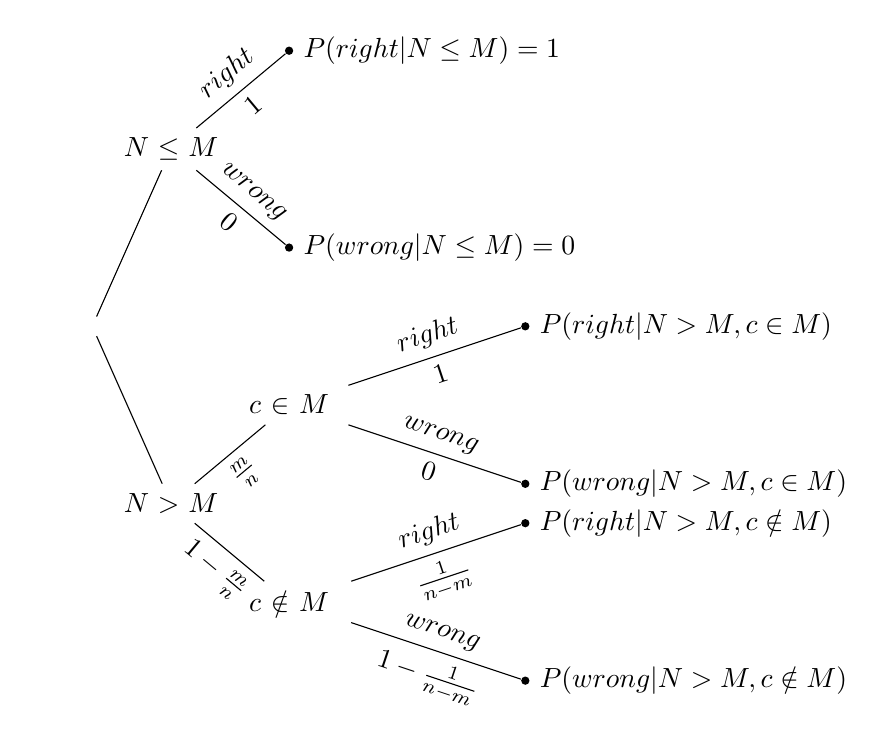
\begin{tikzpicture}[grow=right, sloped]
\node[bag] {}
    child {
        node[bag] {$N > M$}      
            child {
                node[bag] {$c \notin M$}
                    child {
                        node[end, label=right: {$P(wrong | N > M, c \notin M)$}] {}
                        edge from parent
                        node[above] {$wrong$}
                        node[below] {$1 - \frac{1}{n - m}$}
                    }
                    child {
                        node[end, label=right: {$P(right | N > M, c \notin M)$}] {}
                        edge from parent
                        node[above] {$right$}
                        node[below] {$\frac{1}{n - m}$}
                    }
                    edge from parent
                    node[above] {}
                    node[below] {$1 - \frac{m}{n}$}
            }
            child {
                node[bag] {$c \in M$}
                    child {
                        node[end, label=right: {$P(wrong | N > M, c \in M)$}] {}
                        edge from parent
                        node[above] {$wrong$}
                        node[below] {$0$}
                    }
                    child {
                        node[end, label=right: {$P(right | N > M, c \in M)$}] {}
                        edge from parent
                        node[above] {$right$}
                        node[below] {$1$}
                    }
                    edge from parent
                    node[above] {}
                    node[below] {$\frac{m}{n}$}
            }
            edge from parent 
            node[above] {}
            node[below] {}
    }
    child {
        node[bag] {$N \leq M$}        
        child {
            node[end, label=right: {$P(wrong | N \leq M) = 0$}] {}
            edge from parent
            node[above] {$wrong$}
            node[below] {$0$}
        }
        child {
            node[end, label=right: {$P(right | N \leq M) = 1$}] {}
            edge from parent
            node[above] {$right$}
            node[below] {$1$}
        }
        edge from parent         
        node[above] {}
        node[below] {}
    };
<<<<<<< HEAD
\end{tikzpicture}

We seperate two cases. The first is the case where the number of squares on screen can all be remembered by the subject ($N \leq M$).
\begin{align}
&&P(right | N \leq M) &= 1 \\
&&P(wrong | N \leq M) &= 0 \\
\end{align}
The second case is the more interesting one, where not all squares can be remembered ($N > M$).
\begin{align}
&&P(right | N > M, c \in M) &= \frac{M}{N} \\
&&P(wrong | N > M, c \in M) &= 0 \\
&&P(right | N > M, c \notin M) &= (1 - \frac{M}{N}) \frac{1}{N-M} \\
&&P(wrong | N > M, c \notin M) &= (1 - \frac{M}{N}) (1 - \frac{1}{N-M})
\end{align}
We now add up the cases where the subject  gets the right answer.
\begin{align}
P(right) &= \frac{M}{N} + (1 - \frac{M}{N}) \frac{1}{N-M} = \frac{M+1}{N}
\end{align}

=======
\end{tikzpicture}
>>>>>>> 0e0eea4122e3b3789f5f44bed195346e3c9756c1
